
\subsubsection{07.10.14}

\begin{enumerate}
	\item The time of beginning and ending of the meeting:
	17:00 - 21:30
	\item Purposes of the meeting:
	\begin{enumerate}
	  \item Writing a program to control the robot by joystick.
	  
	  \item Beginning of creating the lift.
	  
    \end{enumerate}
	\item Work, that has been done:
	\begin{enumerate}
	  \item Today control of the robot by joystick was implemented. Motor control was carried out by the left stick. During the tests it was found that when a small current was supplied on motors, they could not be rotated and too much loud have been to motors. In this regard it was decided to put a limit to the supply of too small signal.
	  
      \item  In order to raise the basket to 120 cm, it was decided to assemble two guides each of which consists of four furniture rails: two by 30 cm and two by 35 cm. Thus the lifting height is 130 cm. The guides were installed on the robot.
      
      \begin{figure}[H]
      	\begin{minipage}[h]{0.31\linewidth}
      		\center{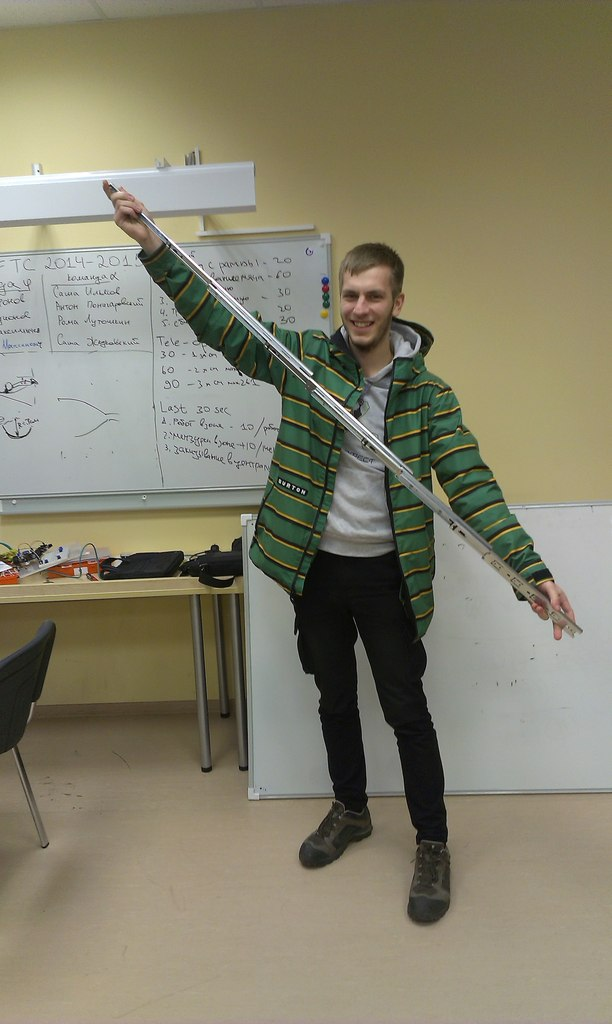
\includegraphics[scale=0.25]{days/07.10.14/images/01}}
      	\end{minipage}
      	\hfill
      	\begin{minipage}[h]{0.31\linewidth}
      		\center{
\includegraphics[scale=0.2]{days/07.10.14/images/02}}
      	\end{minipage}
      	\hfill
      	\begin{minipage}[h]{0.31\linewidth}
      		\center{
\includegraphics[scale=0.25]{days/07.10.14/images/03}}
      	\end{minipage}
      	\caption{Guides for the lift}
      \end{figure}
      
      \item It was decided to install a lift in the central part of the robot. Electronics was installed in the rear part and protected from damage by the lifting mechanism. Some space was left for the bucket in front of the robot. 
       
      \item Bucket is lowered inside the robot so this position is protected from the collision. But in this case, the question how the balls will get into the bucket arises if it will be located inside the robot. It was decided to increase the distance between the floor and the bottom of the front frame of beam to 7 cm so that a big ball could go. This has been achieved by turning the motor around in their mounts. In addition, the decision to increase clearence is increased the stability of the robot.
      
      \begin{figure}[H]
      	\begin{minipage}[h]{1\linewidth}
      		\center{
\includegraphics[scale=0.3]{days/07.10.14/images/04}}
      		\caption{Increase clearance} 
      	\end{minipage}
      \end{figure}
        
      \item In front of the robot it was decided to install a soft brush, such as those installed on the snow machines that will rotate and capture balls. In the case when the robot has collected a maximum number of balls, the operator can stop the rotation of the brushes so other balls will not accidentally get into the bucket.
      
      \begin{figure}[H]
      	\begin{minipage}[h]{0.47\linewidth}
      	    \center{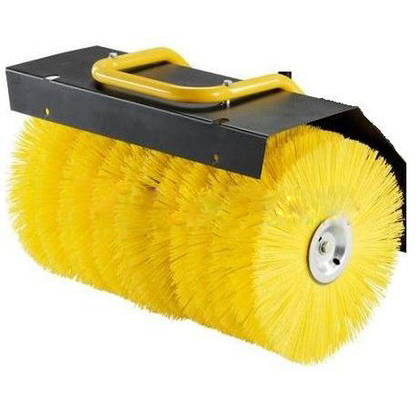
\includegraphics[scale=0.3]{days/07.10.14/images/05}}
      	\end{minipage}
      	\hfill
      	\begin{minipage}[h]{0.47\linewidth}
      		\center{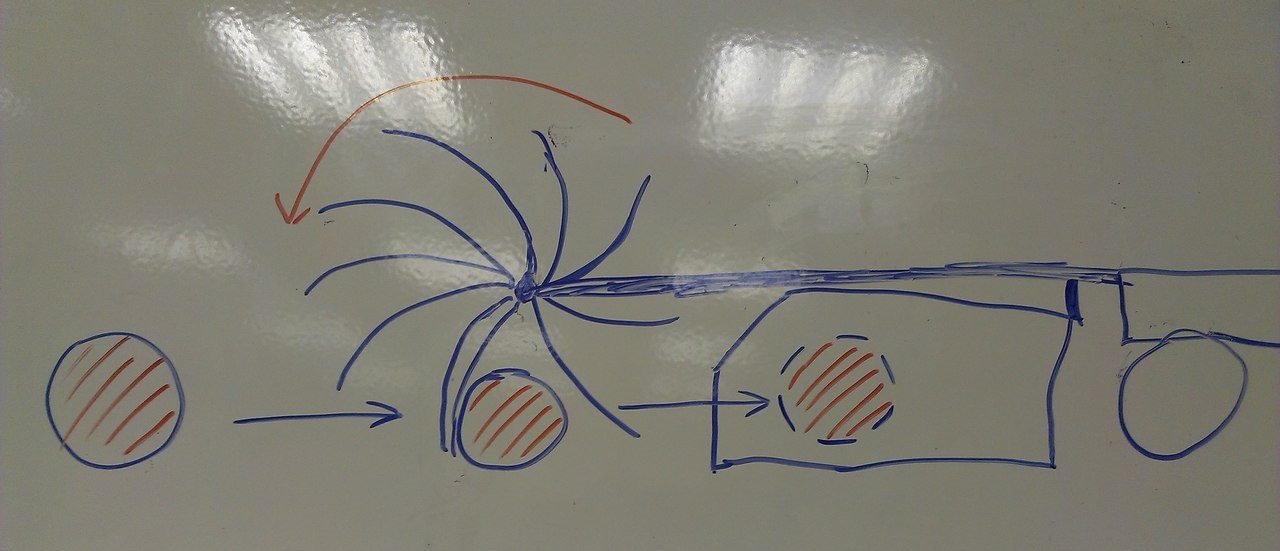
\includegraphics[scale=0.2]{days/07.10.14/images/06}}
      	\end{minipage}
      	\vfill
      	\begin{minipage}[h]{0.47\linewidth}
      	  \center appearance
        \end{minipage}
        \hfill
      	\begin{minipage}[h]{0.47\linewidth}
      	  \center The principle of operation
        \end{minipage}
      	\caption{The idea to capture balls}
      \end{figure}
      
    \end{enumerate}
    
	\item Results:  
	\begin{enumerate}
	  \item It was implemented a simple program to control the robot.
	  
      \item  It was created and assigned rails for the lift.
      
      \item  Battery and motor drivers are properly fixed on the robot. NXT block has not been fixed, as it requirs periodically to removed for battery replacement.
      
      \item Clearance of the robot has been increased.
      
    \end{enumerate}
    
	\item Tasks for the next meetings:
	\begin{enumerate}
	  \item To finish the program of the robot control.
	  
	  \item To implement control of the robot by Bluetooth.
	  
	  \item To create a mechanism for moving apart guides.
	  
    \end{enumerate}     
\end{enumerate}
\fillpage
